\section{POLARIZACIÓN}
\subsection{Ondas Linealmente Polarizadas}

\begin{frame}{POLARIZACIÓN}
    \framesubtitle{Ondas Linealmente Polarizadas}
    Cuando una onda tiene desplazamientos sólo en una dirección, se dice que está linealmente polarizada en esa dirección.
    \begin{figure}
        \centering
        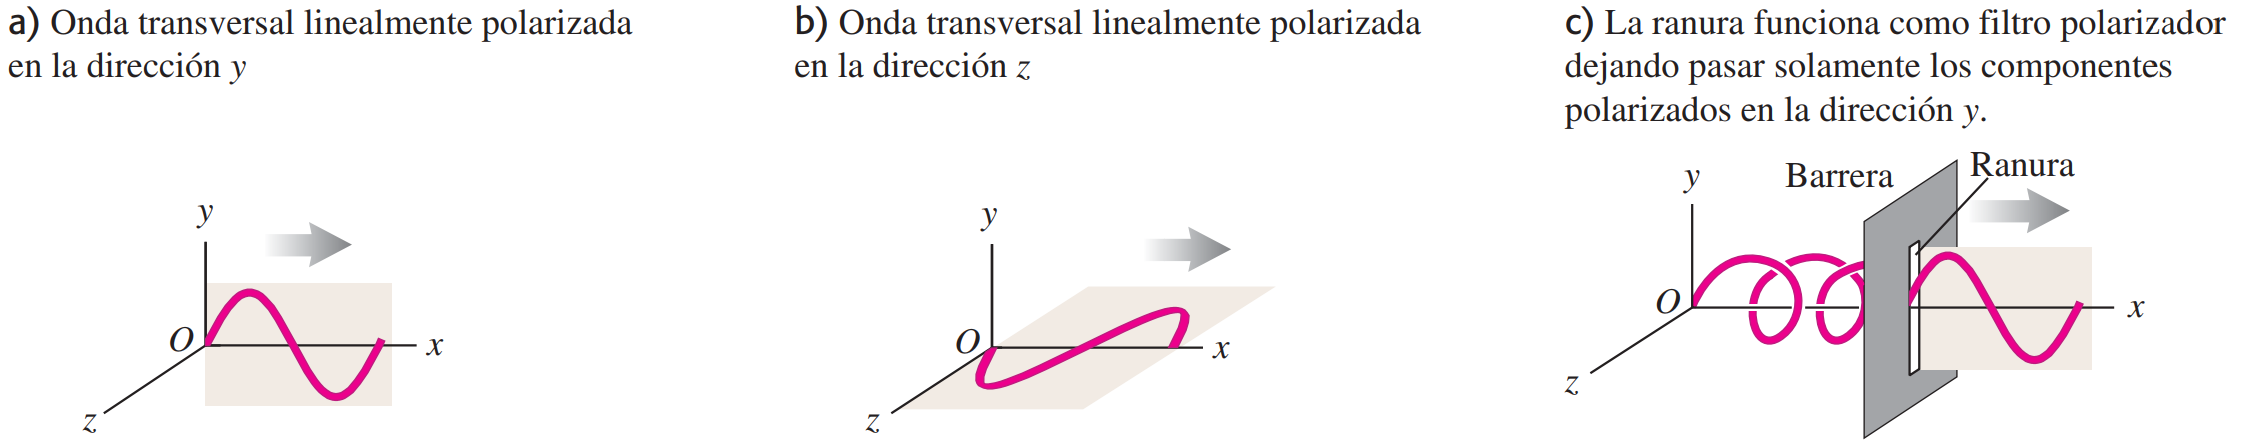
\includegraphics[scale=0.1815]{mari/m_linealpolari.PNG}
        \caption{Ondas linealmente polarizadas\footnotemark{}.}
        \footnotetext{\bibentry{sears}}
    \end{figure}
\end{frame}
%%%%%%%%%%%%%%%%%%%%%%%%%%%%%%%%%%%%%%%
\subsection{Dirección de Polarización}
\begin{frame}{POLARIZACIÓN}
    \framesubtitle{Dirección de Polarización}
    Siempre se define la dirección de polarización de una onda electromagnética como la dirección del vector de campo eléctrico \textbf{E}.
    \begin{equation}
        \overrightarrow{E}(x,t)=\jhat E_{max}\cos\left({kx-\omega t}\right)
    \end{equation}
    \begin{equation}
        \overrightarrow{B}(x,t)=\khat B_{max}\cos\left({kx-\omega t}\right)
    \end{equation}
\end{frame}
%%%%%%%%%%%%%%%%%%%%%%%%%%%%%%%%%%%%%%%%%%
\subsection{Filtros Polarizadores}
\begin{frame}{POLARIZACIÓN}
    \framesubtitle{Filtros Polarizadores}
    El filtro Polaroid incorpora sustancias que presentan dicroísmo, la absorción selectiva en la que una de las componentes polarizadas se absorbe con mucha más intensidad que la otra. Transmite el 80\% o más de la intensidad de una onda que esté polarizada en forma paralela a cierto eje en el material, llamado eje de polarización, pero sólo el 1\% o menos de las ondas polarizadas perpendiculares a ese eje\footnote{\bibentry{sears}.}.

        \begin{figure}
        	\centering
        	\begin{subfigure}[H]{0.4\textwidth}
                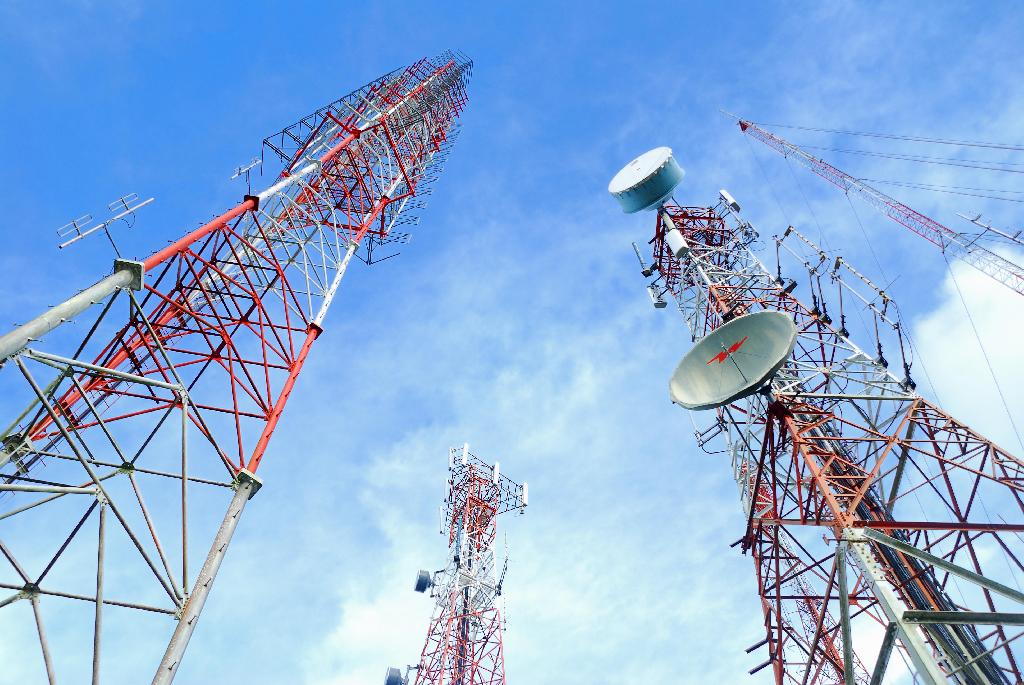
\includegraphics[width=\linewidth]{mari/Antenas.jpg}
                \caption{Antenas telecomunicaciones\footnotemark{}.}
        	\end{subfigure}
            \hspace{2mm}
            \begin{subfigure}[H]{0.32\textwidth}
            	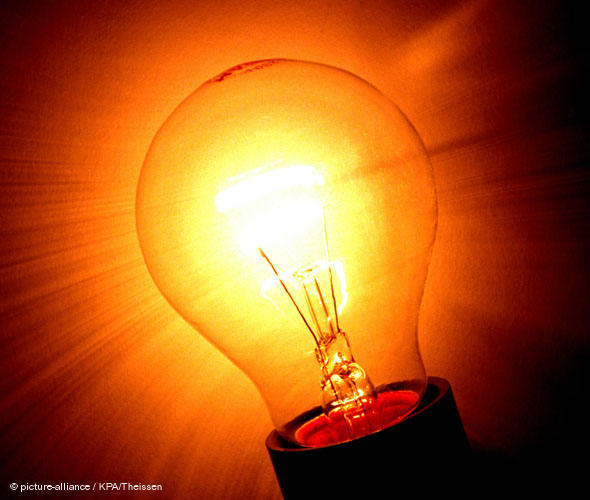
\includegraphics[width=\linewidth]{mari/bombilla.jpg}
                \caption{Bombilla\footnotemark{}.}
            \end{subfigure}
        \end{figure}
        \addtocounter{footnote}{-1}
        \footnotetext{\vspace{-1mm}\bibentry{antena}.}
        \addtocounter{footnote}{1}
        \footnotetext{\bibentry{bombilla}.}
\end{frame}

\begin{frame}{POLARIZACIÓN}
    \framesubtitle{Filtros Polarizadores}
    \begin{figure}[H]
        \centering
        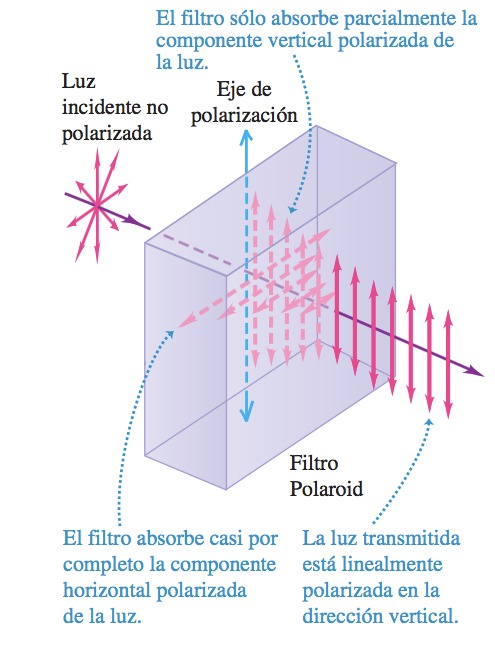
\includegraphics[scale=0.26]{mari/m_filtropolari.jpeg}
        \caption{Filtro polarizador\footnotemark{}.}
    \end{figure}
    \vspace{-10mm}\footnotetext{\bibentry{sears}.}
\end{frame}
%%%%%%%%%%%%%%%%%%%%%%%%%%%%%%%%%%%%%%%%%%%%

\subsection{Ley de Malus}
\begin{frame}{POLARIZACIÓN}
    \framesubtitle{Ley de Malus}
    \begin{figure}[H]
        \centering
        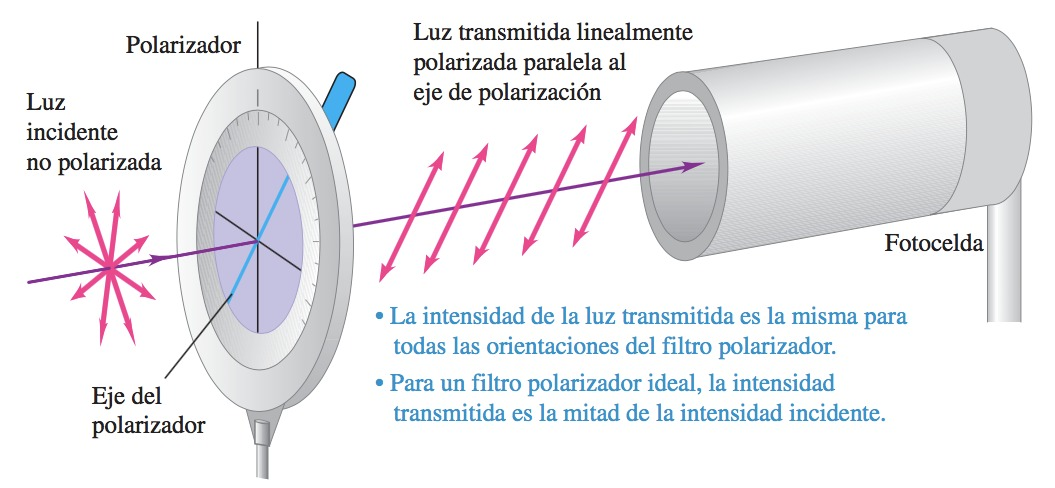
\includegraphics[scale=0.25]{mari/m_malus1.jpeg}
    \end{figure}
    La luz incidente es una mezcla aleatoria de todos los estados de polarización, las componentes paralela y perpendicular al eje de polarización son iguales en promedio, por lo que sólo se transmite la mitad de la intensidad incidente\footnote{\bibentry{sears}}.
\end{frame}

\begin{frame}{POLARIZACIÓN}
    \framesubtitle{Ley de Malus}
    \begin{figure}[H]
        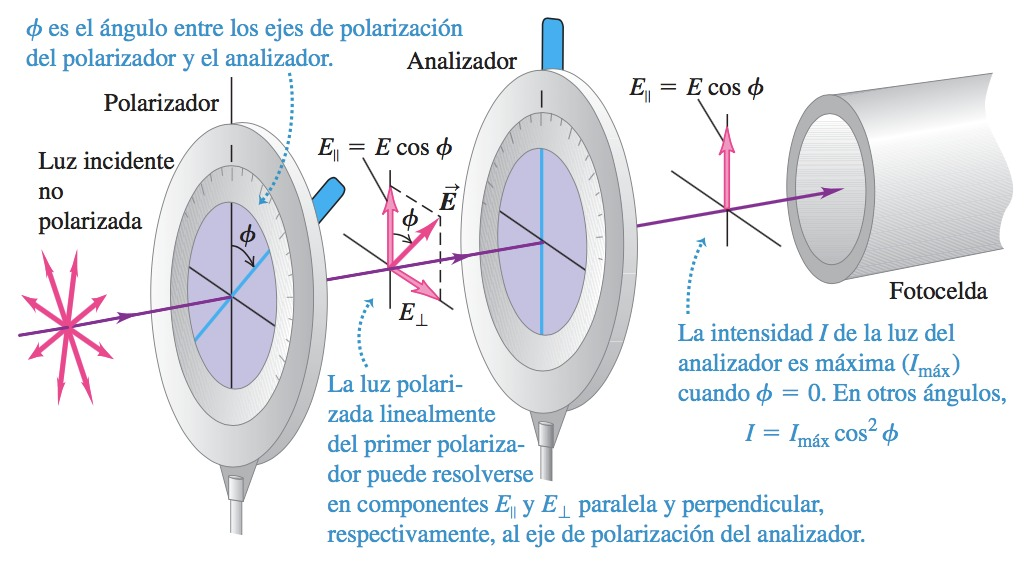
\includegraphics[scale=0.25]{mari/m_malus2.jpeg}
        \caption{Intesidad de luz polarizada\footnotemark{}.}
    \end{figure}
    \footnotetext{\bibentry{sears}}
\end{frame}

\begin{frame}{POLARIZACIÓN}
    \framesubtitle{Ley de Malus}
    Para determinar la intensidad de la luz que sale del analizador debemos saber que la intensidad de una onda electromagnética es proporcional al cuadrado de la amplitud de la onda.
    \begin{equation}
        \begin{split}
            I&=S_{med}=\frac{E_{max}B_{max}}{2\mu_0}=\frac{E_{max}^2}{2\mu_0 c}
            \\&=\frac{1}{2}\sqrt{\frac{\epsilon_0}{\mu_0}}E_{max}^{2}=\frac{1}{2}\epsilon_0 cE_{max}^2
        \end{split}
    \end{equation}

    La razón entre la amplitud trasmitida y la incidente es cos phi, por lo que la razón entre la intensidad transmitida y la incidente es $\cos^2{\phi}$. Así, la intensidad de la luz transmitida a través del analizador es\footnote{\bibentry{sears}}:
    \begin{equation}
        I = I_{max}\cos^2{\phi}
    \end{equation}
\end{frame}
%%%%%%%%%%%%%%%%%%%%%%%%%%%%%%%%%%%%%%%%%%%
\subsection{Polarización por Reflexión}

    %Para cierto ángulo particular de incidencia, llamado el ángulo de polarización, $\theta_p$, la luz cuyo \textbf{E} yace en el plano de incidencia no se refleja en absoluto, sino que se refracta por completo. A ese mismo ángulo de incidencia, la luz cuyo \textbf{E} es perpendicular al plano de incidencia se refleja parcialmente y la otra parte se refracta.
    %\footnotetext{\bibentry{sears}.}


\begin{frame}{POLARIZACIÓN}
    \framesubtitle{Polarización por Reflexión}
    En 1812 el científico británico Sir David Brewster descubrió que cuando el ángulo de incidencia es igual al ángulo de polarización $\theta_p$, el rayo reflejado y el rayo refractado son perpendiculares entre sí.
    \begin{equation}
        \tan{\theta_p}=\frac{n_b}{n_a}
    \end{equation}
    \begin{figure}
        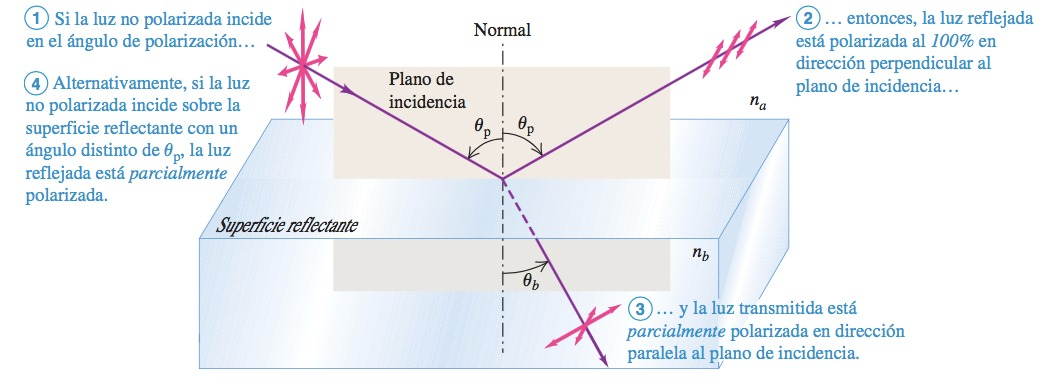
\includegraphics[scale=0.2775]{mari/m_reflex.jpeg}
        \caption{Ley de Brewster para el ángulo de polarización\footnotemark{}.}
    \end{figure}
    \vspace{-1cm}\footnotetext{\bibentry{sears}.}
\end{frame}
